Let's start from a matlab-coder's perspective.
We can, of course, build up a library of functions to fulfill all our basic needs (integration, curve fitting, etc.), and so we can also do this in Python.
However, if we did so in the obvious way, we would have to keep track of error propagation, which index dimensions corresponded to which axes, what the axes were before and after Fourier transformation, all by ourselves.
This is where we can take advantage of the object oriented nature of python.

For instance, let's take simple Fourier transformation.
For non-OO programming, we need to create separate variables to deal with the data and axis,
    and to deal with them separately, as illustrated:
    \begin{center}
        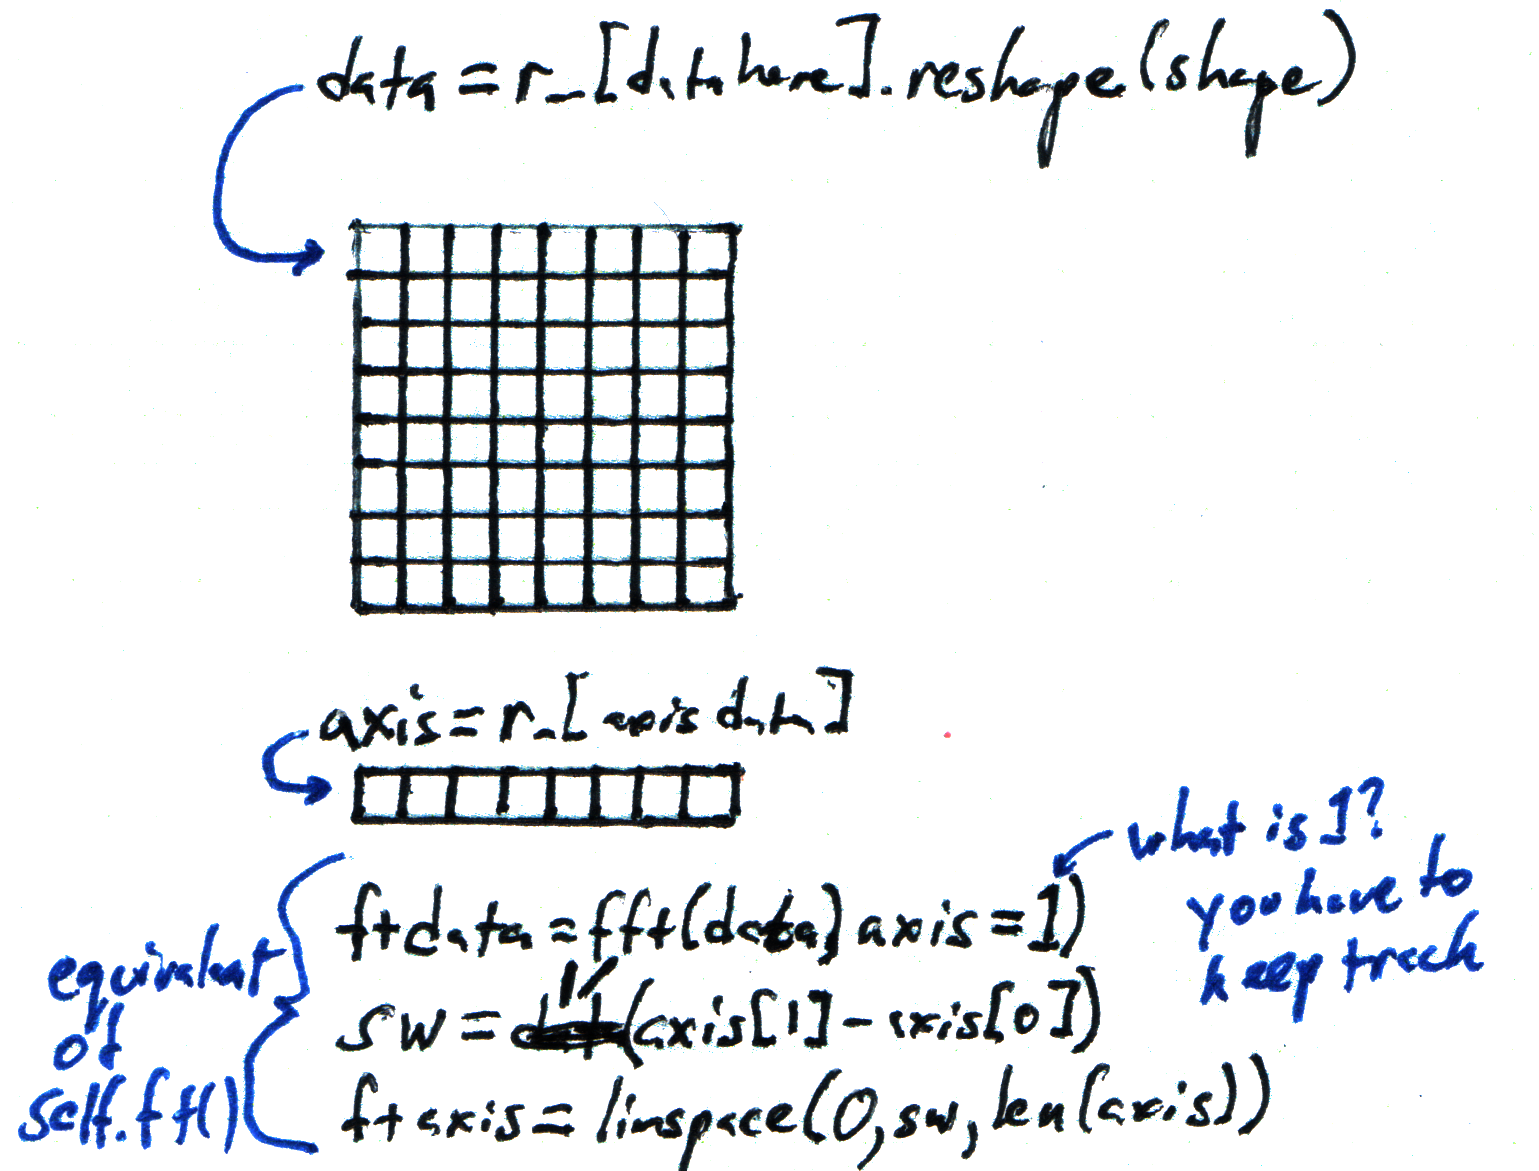
\includegraphics[width=2.565in]{sketches/code_expl_nonobj.png}
    \end{center}
However, with OO programming, we load all our data into the same box.
We define a special type of object, which we call ``nddata.''
The shape or ``structure'' of this nddata container (shown below) automatically takes care
    of properly organizing our data,
    so that we can
    manipulate the data in any way we like
    (i.e. ft, sum, diff, integrate, convolve, addition, subtraction, etc.)
    while {\it transparently handling} the propagation of errors, reassigning of axes, etc.
    \begin{center}
        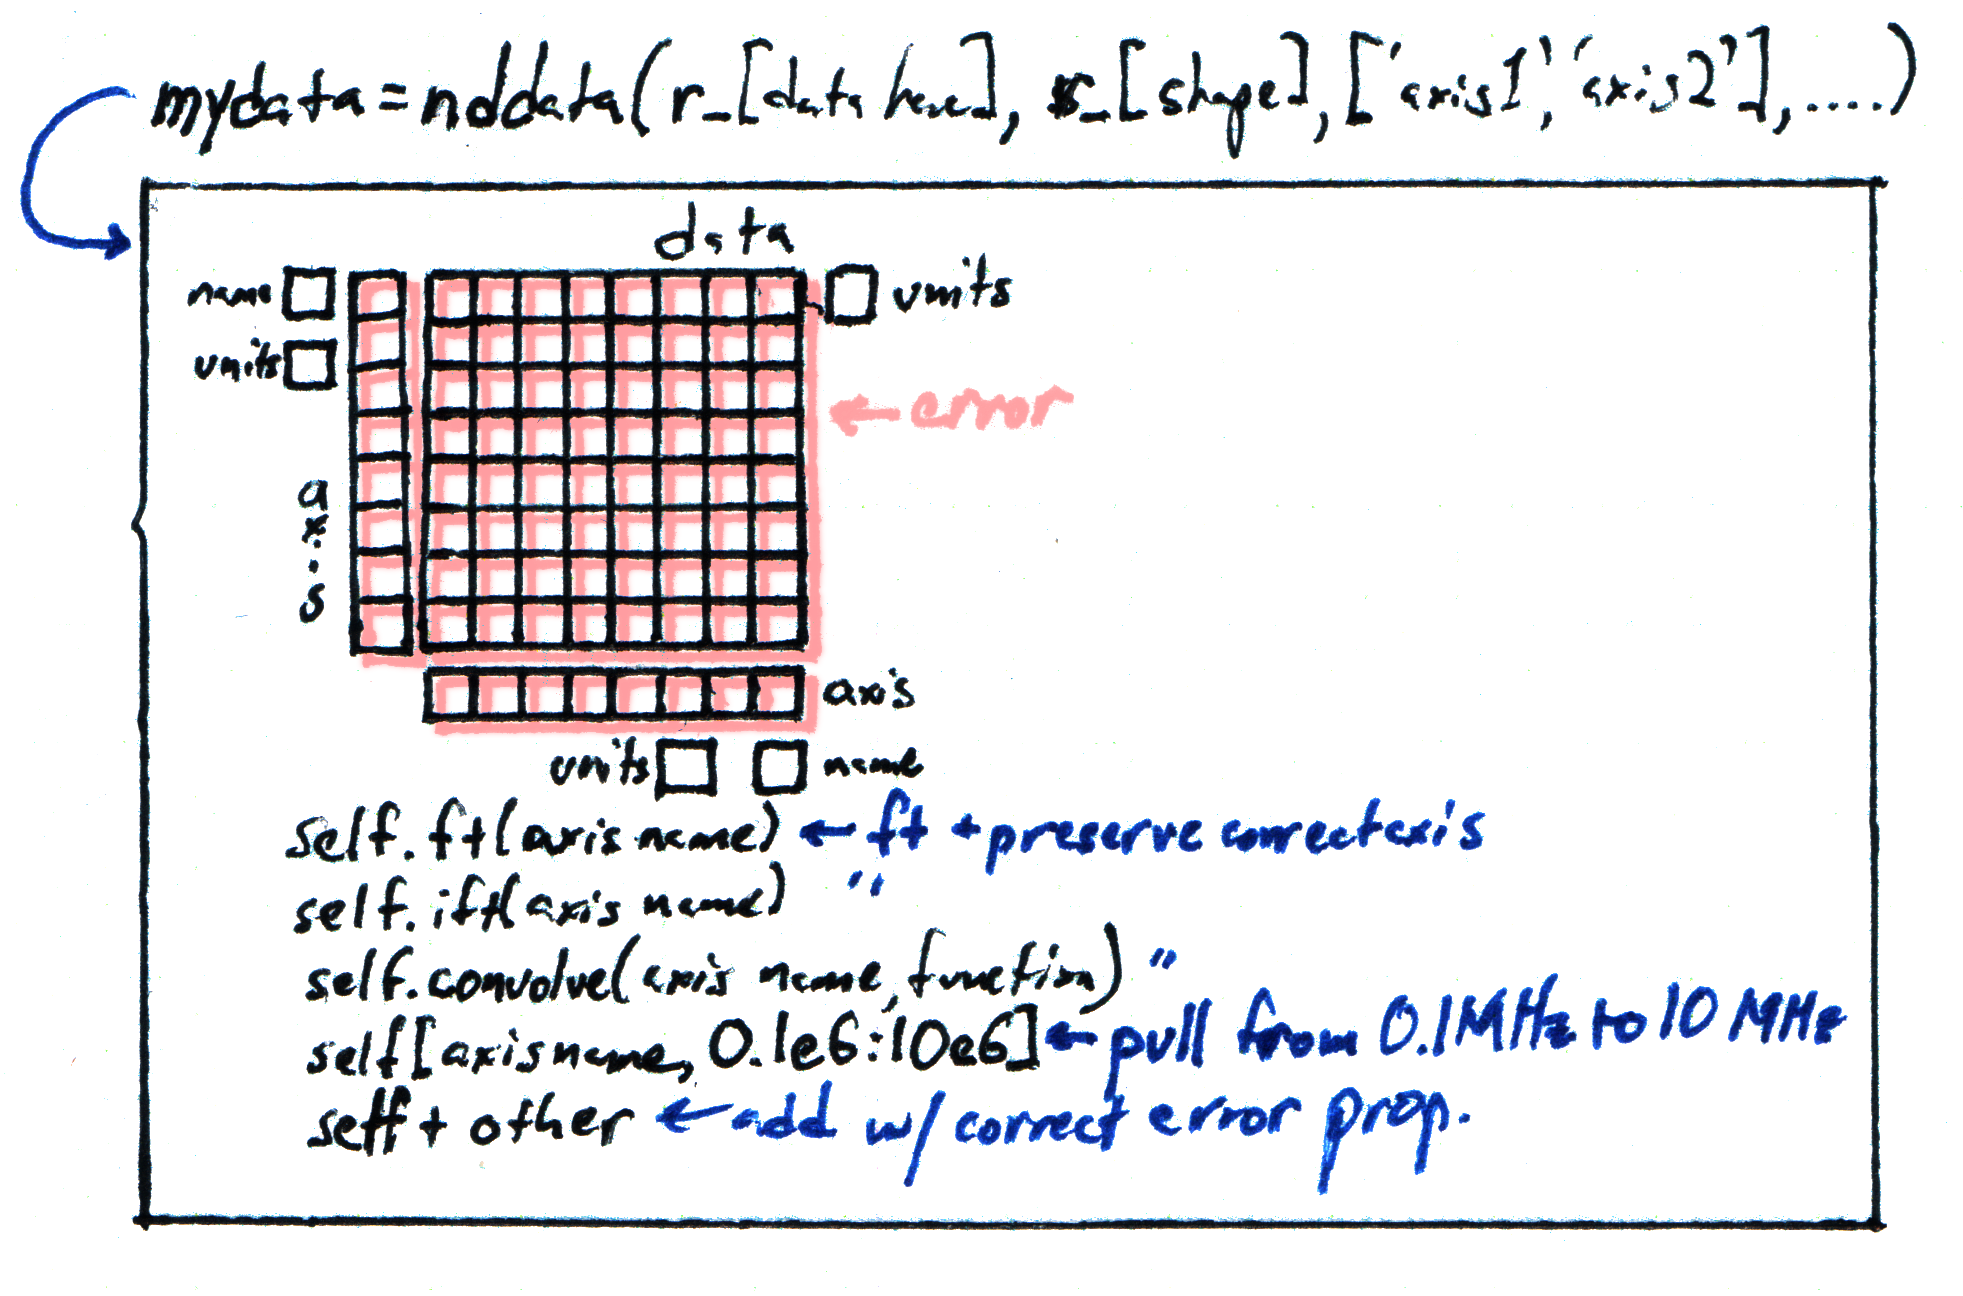
\includegraphics[width=3.272in]{sketches/code_expl_obj.png}
    \end{center}


Then we can define a bunch of libraries that allow us to:
\begin{itemize}
    \item read from standard NMR formats into an nddata object
    \item catalog nddata objects in an HDF5 (a standard format for storing large amounts of data) file.
    \item perform common tasks for us (integration, curve fitting, etc.) that work on nddata objects 
    \item plotting nddata objects, and automatically showing the associated errors and axes 
\end{itemize}

The current version of the DNP code that people are using is merely a user-end function that uses these libraries.
What's more important is that we have a system that allows us to do very controlled analysis of our raw data, but which can easily handle such tedious issues as error propagation, axes, etc, without the need for us to write extra lines of code.
It is not for everyone -- it requires knowing how to code, as well as learning the specific libraries that I've added -- but I hope to convince with several examples that the payoff is worthwhile.

(continued on next page\ldots)

\vspace*{\fill}\pagebreak
Let's take an example, to make things easier.
Let's say we want (without any bells and whistles) to calculate our signal enhancement,
    along with the associated noise.
We would follow this procedure, where each variable
    that the programmer must name and keep track of has been highlighted
    with a different color.

    \quad

\begin{minipage}{\textwidth}
    \begin{tabular}{p{0.2\textwidth}|p{0.3\textwidth}c|p{0.3\textwidth}c}
            {\bf the general procedure.}
            &
            {\bf In Matlab or unmodified Python, we would have to follow these steps:}
            &
            = \# steps
            &
            {\bf However, by using nddata objects, we can do the same thing with the following steps:}
            &
            = \# steps
            \\ \hline\hline
            $\bullet$ Open the raw data.
            &
            \begin{minipage}{0.3\textwidth}
                $\bullet$ Load the raw {\color{red} data} from the NMR data file.

                $\bullet$ Determine the {\color{blue} timestep} from the NMR data files.
            \end{minipage}
            &
            2
            &
            \begin{minipage}{0.3\textwidth}
            $\bullet$ Load the raw data, and associated time information from the NMR data files directly into an {\color{red} nddata object}.
            \end{minipage}
            &
            1
            \\ \hline
            $\bullet$ Fourier transform.
            &
            \begin{minipage}{0.3\textwidth}
                $\bullet$ Fourier transform the {\color{red} data}.
            
                $\bullet$ Use the {\color{blue} timestep} to calculate the {\color{green} frequency axis}.
            \end{minipage}
            &
            2
            &
            \begin{minipage}{0.3\textwidth}
                $\bullet$ Fourier transform the {\color{red} data}.
            \end{minipage}
            &
            1
            \\ \hline
            \begin{minipage}{0.2\textwidth}
                $\bullet$ Store the microwave power level associated with each scan.
            \end{minipage}
            &
            \begin{minipage}{0.3\textwidth}
                $\bullet$ Save the {\color{violet} power levels } in an array. 
            \end{minipage}
            &
            1
            &
            \begin{minipage}{0.3\textwidth}
                $\bullet$ Attach the power levels directly to the {\color{red} nddata object}.
            \end{minipage}
            &
            1
            \\ \hline
            $\bullet$ Select a specific frequency range.
            &
            \begin{minipage}{0.3\textwidth}
                $\bullet$ Based on the {\color{green}frequency axis}, determine the {\color{orange} indeces} associated with the frequency range we want to integrate.

                $\bullet$ Select the appropriate {\color{orange} indeces }.
            \end{minipage}
            &
            2
            &
            \begin{minipage}{0.3\textwidth}
                $\bullet$ Slice out the part of the {\color{red} data} that falls within the frequency range we're interested in.
            \end{minipage}
            &
            1
            \\ \hline
            $\bullet$ Plot the signal within this frequency range. 
            &
            \begin{minipage}{0.3\textwidth}
                $\bullet$ Plot the resulting {\color{red} data}.

                $\bullet$ Explicitly specify the {\color{green} frequency labels} for the x-axis.
            \end{minipage}
            &
            2
            &
            $\bullet$ Plot the resulting {\color{red} data}. 
            &
            1
            \\ \hline
            $\bullet$ Integrate the signal.
            &
            \begin{minipage}{0.3\textwidth}
                $\bullet$ Sum the {\color{red} signal}
                and multiply by the {\color{blue} timestep}\footnote{For preserving units, as when calculating signal voltages.}.

                $\bullet$ Determine the {\color{yellow} noise} associated with the integral from the standard deviation.
            \end{minipage}
            &
            2
            &
            \begin{minipage}{0.3\textwidth}
                $\bullet$ Integrate the {\color{red} signal}.

                $\bullet$ Determine the noise associated with the
                integral from the standard deviation,
                and attach to the {\color{red} nddata object}.
            \end{minipage}
            &
            2
            \\ \hline
            \begin{minipage}{0.2\textwidth}
                $\bullet$ Normalize the integral against the unenhanced signal. 
            \end{minipage}
            &
            \begin{minipage}{0.3\textwidth}
                $\bullet$ Determine the index of the {\color{red} data} that taken in the absence of microwave {\color{violet} power}\footnote{For instance, data can be taken with ascending or descending power.}

                $\bullet$ Propagate the {\color{yellow} error} from the division (the {\color{red}data} is also needed for this). 

                $\bullet$ Divide (\ie, normalize) by the appropriate element of the {\color{red} integrated data}.

            \end{minipage}
            &
            3
            &
            \begin{minipage}{0.3\textwidth}
                $\bullet$ Divide (i.e. normalize) by the appropriate element of the {\color{red} integrated data}.
            \end{minipage}
            &
            2
            \\ \hline
            $\bullet$ Plot the result. 
            &
            \begin{minipage}{0.3\textwidth}
                $\bullet$ Plot the {\color{red} data} and {\color{yellow} errors}.

                $\bullet$ Label the x-axis with the appropriate {\color{violet} powers}.
            \end{minipage}
            &
            2
            &
            $\bullet$ Plot the {\color{red} result}. 
            &
            1
            \\\cline{3-3}\cline{5-5}
            \quad
            &
            \quad
            &
            \textbf{16}
            &
            \quad
            &
            \textbf{10}
    \end{tabular}
\end{minipage}
